% =====================================================================
%  LaTeX tables & figures for the deepfake-voice-detection report.
%  Drop into an IEEEtran (or any) document. Required packages:
%     \usepackage{booktabs}   % \toprule \midrule \bottomrule
%     \usepackage{graphicx}   % \includegraphics
%     \usepackage{tabularx}   % wrapping value column in Table IV
%     \usepackage[table]{xcolor}  % OPTIONAL, only for \rowcolor highlighting
%  In a two-column IEEE layout, table*/figure* span both columns.
%  The proposed model's row is emphasised with \textbf; swap for
%  \rowcolor{green!15} if you prefer shading (needs xcolor[table]).
% =====================================================================

% ------------------------- Table I: datasets -------------------------
\begin{table}[t]
\centering
\caption{The three merged source datasets. The combined corpus is
$\sim$97\% fake, so a class-balanced subset (19{,}251 / 19{,}251) was drawn.}
\label{tab:datasets}
\begin{tabular}{@{}llrr@{}}
\toprule
Source (local name) & Description & Real & Fake \\
\midrule
ASVspoof 2021 (DF) & Telephone/codec deepfakes            & 16{,}977 & 441{,}894 \\
Adarsh AD set      & LibriSpeech real + modern-TTS fakes  & 2{,}274  & 2{,}173   \\
MLAAD v5           & Multilingual TTS, $\sim$90 gens (fake only) & 0 & 151{,}446 \\
\midrule
\textbf{Merged}    & Unified manifest                     & \textbf{19{,}251} & \textbf{595{,}513} \\
\bottomrule
\end{tabular}
\end{table}

% ------------------ Table II: in-domain results ----------------------
% Wide (6 columns) -> table* spans both columns in a two-column layout.
\begin{table*}[t]
\centering
\caption{In-domain detection on the speaker-disjoint test set (lower EER is
better). The proposed model roughly halves the best classical baseline's EER,
and the paper's GNB+NMF ``transfer'' step does not help.}
\label{tab:indomain}
\begin{tabular}{@{}llrrrr@{}}
\toprule
Method & Features & EER (\%) & Bal.\ Acc (\%) & F1$_{\text{fake}}$ (\%) & AUC \\
\midrule
\textbf{AttentiveSpecCNN (ours)}     & log-mel           & \textbf{4.81}  & \textbf{93.84} & \textbf{93.49} & \textbf{0.99} \\
Random Forest                        & MFCC              & 11.33 & 87.51 & 87.86 & 0.96 \\
Random Forest                        & GNB+NMF transfer  & 11.89 & 87.60 & 87.83 & 0.95 \\
$k$-Nearest Neighbours               & MFCC              & 13.15 & 85.46 & 86.13 & 0.92 \\
Logistic Regression                  & GNB+NMF transfer  & 14.78 & 84.73 & 84.09 & 0.92 \\
$k$-Nearest Neighbours               & GNB+NMF transfer  & 15.05 & 83.93 & 84.67 & 0.91 \\
Logistic Regression                  & MFCC              & 15.52 & 84.33 & 84.17 & 0.91 \\
Gaussian Naive Bayes                 & GNB+NMF transfer  & 23.93 & 76.72 & 75.77 & 0.87 \\
Gaussian Naive Bayes (paper headline)& MFCC              & 26.69 & 73.05 & 71.75 & 0.81 \\
\bottomrule
\end{tabular}
\end{table*}

% ---------------- Table III: cross-dataset results -------------------
\begin{table}[t]
\centering
\caption{Leave-one-source-out generalisation. In-domain success does not
transfer to a fully unseen source. MLAAD has no real audio, so only the
fake-detection rate on unseen generators is reportable.}
\label{tab:cross}
\begin{tabular}{@{}lllr@{}}
\toprule
Held-out test source & Trained on & Metric & Result \\
\midrule
\textit{(ref.) In-domain} & all three      & EER / AUC & \textbf{4.81\% / 0.99} \\
ASVspoof 2021             & ds2 + MLAAD    & EER / AUC & 44.9\% / 0.56 \\
dataset\_2                & ASV + MLAAD    & EER / AUC & 57.5\% / 0.42 \\
MLAAD                     & ASV + ds2      & fake-recall & 48.4\% \\
\bottomrule
\end{tabular}
\end{table}

% ---------------- Table IV: model & training config ------------------
\begin{table}[t]
\centering
\caption{Audio front-end, model, and training configuration for the proposed
AttentiveSpecCNN.}
\label{tab:config}
\begin{tabularx}{\columnwidth}{@{}lX@{}}
\toprule
Setting & Value \\
\midrule
Sample rate / channels & 16\,kHz, mono \\
Clip length            & 4\,s (64{,}000 samples); pad, else random crop (train) / center crop (eval) \\
Log-mel spectrogram    & 80 mel bands, $n_\text{fft}{=}400$, hop${=}160$ $\rightarrow$ $80{\times}401$ \\
CNN backbone           & 4 conv blocks, channels 16/32/64/128, $3{\times}3$ conv + BN + ReLU + $2{\times}2$ max-pool \\
Pooling                & frequency mean, then temporal attention (softmax over time) \\
Classifier head        & Linear $128{\to}64$, ReLU, dropout 0.3, Linear $64{\to}2$ \\
Parameters             & $\approx$106{,}000 \\
Optimiser / schedule   & Adam, lr $10^{-3}$, ReduceLROnPlateau ($\times0.5$, patience 2) \\
Loss                   & cross-entropy, inverse-frequency class weights \\
Batch / epochs         & 64 / 15, best-val-EER checkpoint \\
Hardware               & single NVIDIA RTX 3080 \\
\bottomrule
\end{tabularx}
\end{table}

% ------------------------- Figures -----------------------------------
\begin{figure}[t]
\centering
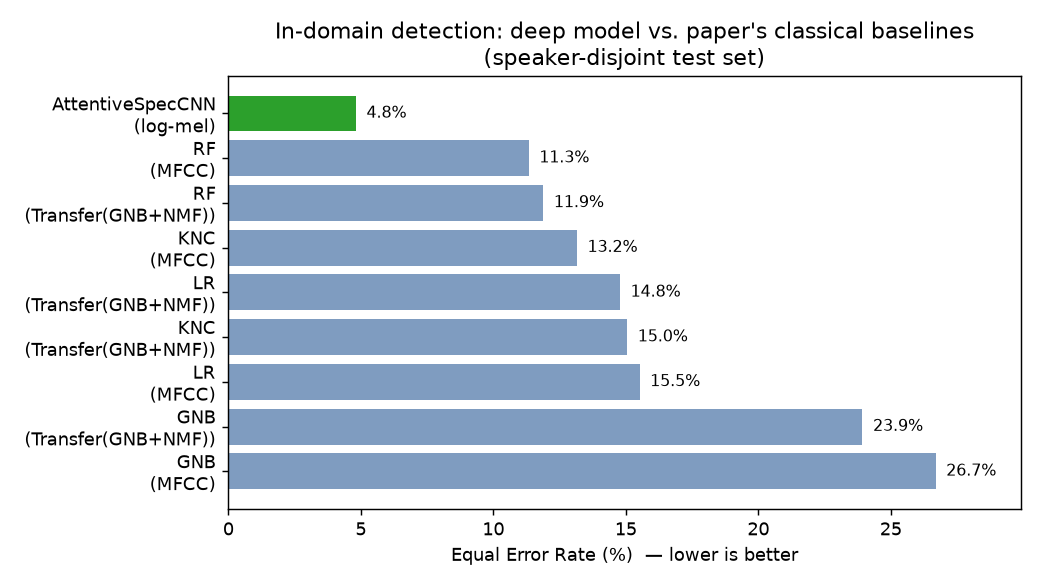
\includegraphics[width=\columnwidth]{fig_method_comparison.png}
\caption{Equal Error Rate by method on the speaker-disjoint test set. The
proposed AttentiveSpecCNN roughly halves the best classical baseline's EER.}
\label{fig:method}
\end{figure}

\begin{figure}[t]
\centering
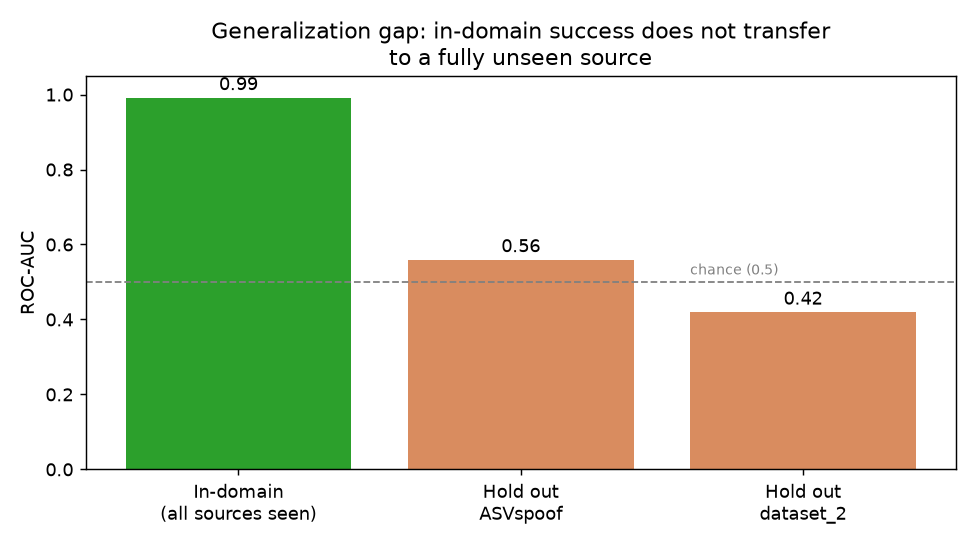
\includegraphics[width=\columnwidth]{fig_cross_dataset.png}
\caption{In-domain vs.\ held-out ROC-AUC. Performance collapses to (or below)
chance when the test source is entirely unseen during training.}
\label{fig:cross}
\end{figure}

% Wide 3-panel explanation -> figure* spans both columns.
\begin{figure*}[t]
\centering
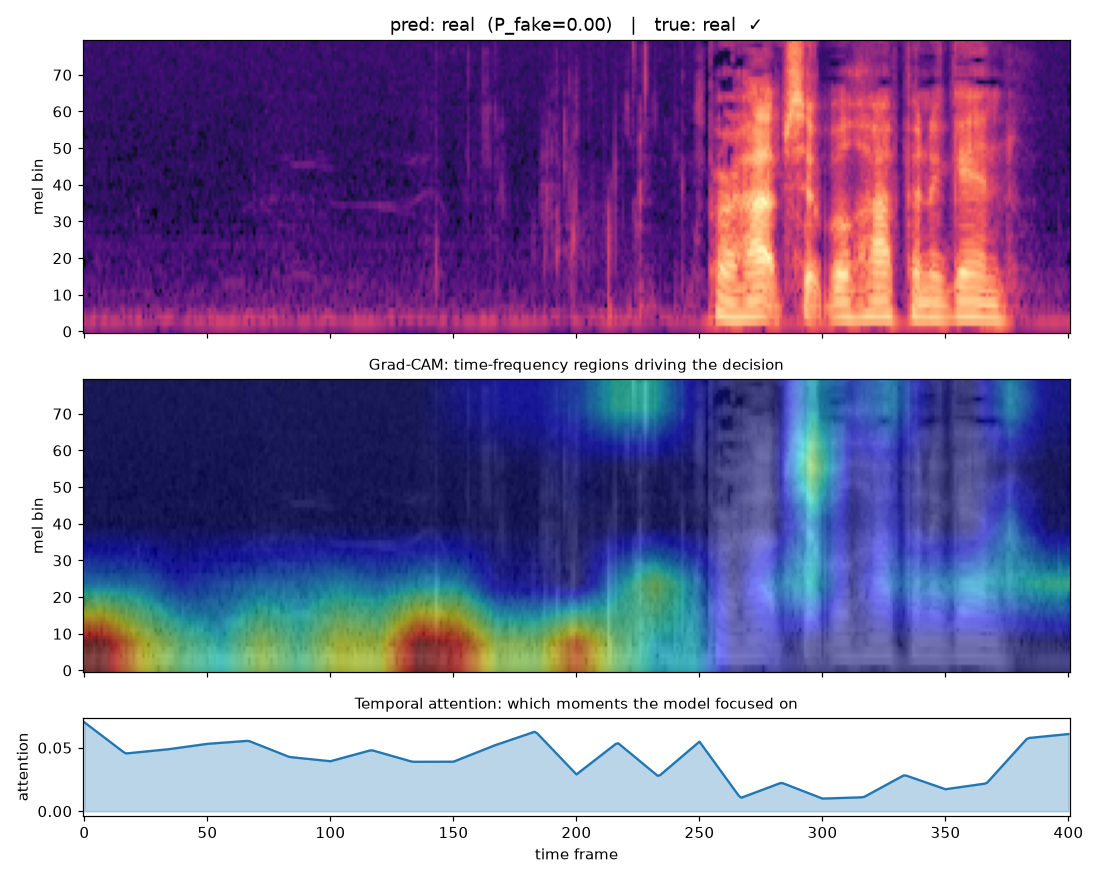
\includegraphics[width=0.82\textwidth]{explanations/real_DF_E_2774626.flac.png}
\caption{Explanation for a correctly-identified real clip: log-mel spectrogram
(top), Grad-CAM over the time--frequency plane (middle), and the temporal
attention weights (bottom).}
\label{fig:explain}
\end{figure*}
